% !TEX encoding = UTF-8 Unicode
\documentclass[AutoFakeBold,doctype=thesis,printmode=final,blankleft]{sysuthesis}

% 选项说明
% doctype=[thesis|proposal],                  % 可选(默认:thesis),论文类型,thesis 为学位论文,proposal 为开题报告
% printmode=[final|checkmode|blindmode],      % 可选(默认:final),打印模式,final 为终稿,checkmode 为查重模式,blindmode 为盲审模式
% language= [chinese|english] or [zh|en],     % 可选(默认:chinese),论文的主要语言
% blankleft=[true|false],                     % 可选(默认:false),使无内容的偶数页空白
%
% 以下为 ctexbook 文档类的选项,可将此类参数从本模板传递过去
% [openright|openany],                        % 可选(默认:openright),章节分页,奇数页或任意页开始新章
% AutoFakeBold                                % 可选 如果系统中找不到某种字体(如楷书)的粗体,选用 AutoFakeBold 可以作为另一种替代解决方案
% fontset=[fandol|windows|macnew|ubuntu],     % 可选(默认:fandol),字体设置,请根据使用的计算机系统选择适当的选项
% [fleqn|leqno],                              % 可选 公式对齐方式,默认公式居中对齐编号居右对齐,fleqn 选项将使公式居左对齐,leqno 选项将使公式编号居左对齐
% [final|draft],                              % 可选(默认:final),选择 draft 选项将启用草稿模式,这时:
%     1. 文档中的图形(如图片)将以一个框的形式显示,而不是实际的图像内容。
%     2. lstlisting 环境中的内容将不见,只留有标签
%     3. 异常长的行会显示为黑色盒子,需要调整文本以适应页面宽度
% 草稿模式主要用于在编辑文档时快速查看页面布局和图形位置,同时减少编译时间。**注意要将此选项放在第一个**,否则不起作用。

% 设置论文的基本信息,包括题目、作者、专业、导师、学院、摘要和关键词等必要信息
% !TEX root = ./thesis.tex

% 设置基本信息
\sysuset{
    %******************************
    % 注意:配置里面不要出现空行,请删掉空白行或者添加注释符号
    %******************************
    % 中文姓名
    author = {张三},
    % 英文姓名
    author-en = {Zhang San},
    % 中文标题
    title = {中山大学研究生学位论文\LaTeX{}非官方模版},
    % 英文标题
    title-en = {English Title for Sun Yat-sen University Thesis \LaTeX{} Unofficial Template},
    % 中文关键词
    keywords = {天体物理;引力波;黑洞},
    % 英文关键词
    keywords-en = {Astrophysics; Gravitational Wave; Black Holes},
    % 学号
    student-id = {22110000},
    % 专业
    major = {天体物理},
    % 专业英文
    major-en = {Astrophysics},
    % 指导教师姓名
    supervisor = {李四 \quad 副教授},
    % 指导教师英文姓名
    supervisor-en = {Associate Professor \quad Li Si},
    % 学科门类
    discipline = {理学},
    % 学位
    degree = {博士},
    % 校区
    campus = {珠海},
    % 学院
    school = {物理与天文学院},
    % 研究团队
    research-team = {天文团队},
    % 日期
    date = {2022年6月},
}

% 设置模板的一些参数
\sysuset{
    %******************************
    % 注意:配置里面不要出现空行,请删掉空白行或者添加注释符号
    %******************************
    % % 致谢环境名
    % ack-name = {后记},
    % % 附录环境名
    % appendix-name = {附录},
    % % 参考文献名
    % bib-name = {参考文献},
    % % 参考文献表样式,可选项为 numerical(顺序编码制)、author-year(著者-出版年制)
    % bib-style = author-year,
    % 图表等标签和标题的分隔符号,可选项为 none(取消符号)、colon (冒号)、period(句点)、space(空格)、quad(空白)、newline(换行)
    caption-labelsep = space,
    % 算法环境标签和标题的分隔符号
    algorithm-labelsep = {:},
    % % 结论环境名
    % conclusion-name = {结论},
    % % 目录名
    % contents-name = {目\qquad 录},
    % 本模版的主要颜色
    main-color = sysugreen,
    % % 索引名
    % index-name = {索引},
    % % 插图索引名
    % listfigure-name = {插图索引},
    % % 表格索引名
    % listtable-name = {表格索引},
    % % 公式索引名
    % list-equation-name = {公式索引},
    % % 插图标签名
    % figure-name = {图},
    % % 表格标签名
    % table-name = {表},
    % % 插图索引中插图列表的标签名
    % figure-prename-in-lof = {图},
    % % 表格索引中表格列表的标签名
    % table-prename-in-lot = {表},
    % % 插图索引中标签名与标题的距离
    % indent-in-lof = {3.25em},
    % % 表格索引中标签名与标题的距离
    % indent-in-lot = {3.25em},
    % % lstlisting 环境索引名
    % listoflistings-name = {代码索引},
    % % lstlisting 环境标签名
    % lstlisting-name = {代码},
    % % lstlisting 环境的风格,可以查看 listings 宏包的文档自行设置
    % lst-style = {codestyle},
    % % 长表格续表的表头
    % longtable-continued-head = {(续)},
    % % 长表格的表尾
    % longtable-continued-foot = {下页续},
}

% % 图表等标题的对齐方式,可选项为 justified(两端对齐)、centering(居中对齐)、raggedright(左对齐标题)、raggedleft(右对齐标题),详情请看 caption 宏包
% \captionsetup{justification=justified}

% 定义所有的图片文件在 figures 子目录下
\graphicspath{{./figures/}}

% 设置新的latex命令
\newcommand{\dd}{~\mathrm{d}}

% 调用的宏包
\usepackage{longtable}
\usepackage{tablefootnote}
\usepackage{hologo}
\usepackage[edges]{forest}
\forestset{%
    directory/.style={%
        for tree={%
            edge+=thick, 
            folder, 
            font=\ttfamily\zihao{-5},
            grow'=0,
            draw,
        },
    },
}

\begin{document}

% 前置部分
\frontmatter

% 扉页
\maketitle

% 原创性及使用授权说明
\makecopyright

% 中英文摘要
%%
% 摘要信息
% 本文档中前缀"c-"代表中文版字段, 前缀"e-"代表英文版字段
% 摘要内容应概括地反映出本论文的主要内容,主要说明本论文的研究目的、内容、方法、成果和结论。要突出本论文的创造性成果或新见解,不要与引言相 混淆。语言力求精练、准确,以 300—500 字为宜。
% 在摘要的下方另起一行,注明本文的关键词(3—5 个)。关键词是供检索用的主题词条,应采用能覆盖论文主要内容的通用技术词条(参照相应的技术术语 标准)。按词条的外延层次排列(外延大的排在前面)。摘要与关键词应在同一页。
% modifier: 黄俊杰(huangjj27, 349373001dc@gmail.com)
% update date: 2017-04-15
%%

\cabstract{

    摘要应概括论文的主要信息,应具有独立性和自含性,即不阅读论文的全文,就能获得必要的信息。摘要内容一般应包括研究目的、内容、方法、成果和结论,要突出论文的创造性成果或新见解,不要与绪论相混淆。语言力求精练、准确,以300-500字为宜。关键词是供检索用的主题词条,应体现论文特色,具有语义性,在论文中有明确的出处,并应尽量采用《汉语主题词表》或各专业主题词表提供的规范词。关键词与摘要应在同一页,在摘要的下方另起一行注明,一般列3-5个,按词条的外延层次排列(外延大的排在前面)。

}
% 中文关键词(每个关键词之间用“,”分开,最后一个关键词不打标点符号。)
\ckeywords{本科毕业论文,\LaTeX\ 模板,中山大学}

\eabstract{
    % 英文摘要及关键词内容应与中文摘要及关键词内容相同。中英文摘要及其关键词各置一页内。
    The content of the English abstract is the same as the Chinese abstract, 250-400 content words are appropriate. Start another line below the abstract to indicate English keywords (Keywords 3-5).
}
% 英文文关键词(每个关键词之间用,分开, 最后一个关键词不打标点符号。)
\ekeywords{undergraduate thesis, \LaTeX\ template, Sun Yat-Sen University}



% 目录
\tableofcontents
\tableofcontentsen

% % 插图索引
% \listoffigures
% \listoffiguresen

% % 表格索引
% \listoftables
% \listoftablesen

% % 算法索引
% \listofalgorithms

% %代码索引
% \lstlistoflistings
% \listoflstlistingsen

% 主体部分
\mainmatter

% 正文
% !TEX root = ../thesis.tex
\chapter{前\hspace*{1\ccwd}言}
\chapteren{Introduction}

\section{声明}
\sectionen{Declaration}

\sysuthesis{}\footnote{\copyright~\number\year~\href{https://github.com/yanghw8}{yanghw8}\hspace*{2\ccwd}更新时间:\today}是旨在为中山大学熟悉\LaTeX{}语言的研究生提供一个方便易用的学位论文写作模版,其设置的排版格式力求尽可能符合《\href{https://graduate.sysu.edu.cn/sites/graduate.prod.dpcms4.sysu.edu.cn/files/2019-04/%E4%B8%AD%E5%B1%B1%E5%A4%A7%E5%AD%A6%E7%A0%94%E7%A9%B6%E7%94%9F%E5%AD%A6%E4%BD%8D%E8%AE%BA%E6%96%87%E6%A0%BC%E5%BC%8F%E8%A6%81%E6%B1%82.pdf}{中山大学研究生学位论文格式要求}》。首先声明:\strong{本模版不是官方模版,无法保证它完全符合学校的相关要求,在开始使用前,您同意,任何由于本模板而引起的论文格式审查问题与本模板作者无关。}

本模版暂时没有为本科生学位论文设置格式,如果您是本科生,请移步至\href{https://github.com/SYSU-SCC/sysu-thesis}{本科生模版}。如果您没有接触过\LaTeX{},又不打算花费时间和精力来入门,推荐您使用 Microsoft Office 套装来编写您的学位论文。如果您是\LaTeX{}语言的初学者,那么希望以下内容会对您的学习有所帮助。

\section{注意事项}
\sectionen{Notice}

本模版预设的封面、原创性声明及使用授权说明页、摘要页均以物理与天文学院的格式要求为主。如果您所在学院的要求与本模版预设的不同,建议参考以下 \textdagger 项的说明,正文以及参考文献部分各学院的要求应该是一致的。

\begin{itemize}
    \item 一般而言,通常不需要在中英文之间添加额外的空格,但为了代码的可读性(良好的习惯),还是建议在中文字符和 English 字符之间加上空格。
    \item[\textdagger] 对于扉页,如果对本模版预设的扉页不满意,可以使用 \texttt{pdfpages} 宏包中的 \texttt{\char92 includepdf} 命令导入您的扉页的 PDF 文件,例如
\begin{lstlisting}[language=TeX]
% \maketitle
\includepdf{titlepage.pdf}
\end{lstlisting}
    其中 \texttt{titlepage.pdf} 为扉页的 PDF 文件。
    \item[\textdagger] 同样的,对于原创性及使用授权说明页,也可以利用类似的方法:
\begin{lstlisting}[language=TeX]
% \makecopyright
\includepdf{copyrightpage.pdf}
\end{lstlisting}
    其中 \texttt{copyrightpage.pdf} 为扉页的 PDF 文件(可以为签字过后的扫描文件)。
    \item[\textdagger] 对于摘要页,在使用类似上述的命令之后,此外还应将摘要加入目录,因此建议使用以下命令
\begin{lstlisting}[language=TeX]
% %%
% 摘要信息
% 本文档中前缀"c-"代表中文版字段, 前缀"e-"代表英文版字段
% 摘要内容应概括地反映出本论文的主要内容,主要说明本论文的研究目的、内容、方法、成果和结论。要突出本论文的创造性成果或新见解,不要与引言相 混淆。语言力求精练、准确,以 300—500 字为宜。
% 在摘要的下方另起一行,注明本文的关键词(3—5 个)。关键词是供检索用的主题词条,应采用能覆盖论文主要内容的通用技术词条(参照相应的技术术语 标准)。按词条的外延层次排列(外延大的排在前面)。摘要与关键词应在同一页。
% modifier: 黄俊杰(huangjj27, 349373001dc@gmail.com)
% update date: 2017-04-15
%%

\cabstract{

    摘要应概括论文的主要信息,应具有独立性和自含性,即不阅读论文的全文,就能获得必要的信息。摘要内容一般应包括研究目的、内容、方法、成果和结论,要突出论文的创造性成果或新见解,不要与绪论相混淆。语言力求精练、准确,以300-500字为宜。关键词是供检索用的主题词条,应体现论文特色,具有语义性,在论文中有明确的出处,并应尽量采用《汉语主题词表》或各专业主题词表提供的规范词。关键词与摘要应在同一页,在摘要的下方另起一行注明,一般列3-5个,按词条的外延层次排列(外延大的排在前面)。

}
% 中文关键词(每个关键词之间用“,”分开,最后一个关键词不打标点符号。)
\ckeywords{本科毕业论文,\LaTeX\ 模板,中山大学}

\eabstract{
    % 英文摘要及关键词内容应与中文摘要及关键词内容相同。中英文摘要及其关键词各置一页内。
    The content of the English abstract is the same as the Chinese abstract, 250-400 content words are appropriate. Start another line below the abstract to indicate English keywords (Keywords 3-5).
}
% 英文文关键词(每个关键词之间用,分开, 最后一个关键词不打标点符号。)
\ekeywords{undergraduate thesis, \LaTeX\ template, Sun Yat-Sen University}


\addcontentsline{toc}{chapter}{\protect 摘\hspace*{2\ccwd}要}
\addcontentsline{toe}{chapter}{Abstract (In Chinese)}
\includepdf{abstract-zh.pdf}
\addcontentsline{toc}{chapter}{ABSTRACT}
\addcontentsline{toe}{chapter}{Abstract (In English)}
\includepdf{abstract-en.pdf}
\end{lstlisting}
    其中 \texttt{abstract-zh.pdf} 和 \texttt{abstract-en.pdf} 分别为中英文摘要页的 PDF 文件。
    \item 对于插图和表格的标题,本模版推荐使用 \texttt{bicaption} 宏包的 \texttt{\char92 bicaption} 命令,具体用法为:
\begin{lstlisting}[language=TeX]
\bicaption[中文短标题]{中文标题}[英文短标题]{英文标题}
\end{lstlisting}
    其中,短标题在插图索引或者表格索引中展示,而标题则在插图下方或者表格上方展示,见\autoref{fig:hexbin}示例。
    \item 在图表标题中,出现了引用文献后字号变回正文字号的问题,该问题有一个简单的解决方法,即使用 \texttt{\{\char92 cite\{key\}\}} 来避免上述问题发生。\strong{在弃用 \texttt{cite} 宏包之后,该问题似乎已经解决了。}
\end{itemize}

\section{使用说明}
\sectionen{Readme}

硕士论文不要求中英双目录和图表双标题,使用时仅使用
\begin{itemize}
    \item \texttt{\char92 chapter\{\}}
    \item \texttt{\char92 section\{\}}
    \item \texttt{\char92 subsection\{\}}
    \item \texttt{\char92 caption\{\}}
\end{itemize}
即可。博士使用
\begin{itemize}
    \item \texttt{\char92 chapter\{\}}、 \texttt{\char92 chapteren\{\}}
    \item \texttt{\char92 section\{\}}、 \texttt{\char92 sectionen\{\}}
    \item \texttt{\char92 subsection\{\}}、 \texttt{\char92 subsectionen\{\}}
    \item \texttt{\char92 bicaption\{\}\{\}}
\end{itemize}
以显示双语效果。此外,如果需要展示目录和索引,请直接使用\autoref{tab:listof}中的命令来打开。
\begin{table}[!htp]
    \zihao{5}
    \bicaption{目录索引}
    {Table of contents and  List of X}
    \label{tab:listof}
    \centering
    \begin{tabular}{ll}
        \toprule
        索引    & 命令 \\
        \midrule
        中文目录    &  \texttt{\char92 tableofcontents} \\
        英文目录    &  \texttt{\char92 tableofcontentsen} \\
        中文插图索引    &  \texttt{\char92 listoffigures} \\
        英文插图索引    &  \texttt{\char92 listoffiguresen} \\
        中文表格索引   &  \texttt{\char92 listoftables} \\
        英文表格索引   &  \texttt{\char92 listoftablesen} \\
        算法索引   &  \texttt{\char92 listofalgorithms} \\
        中文代码索引   &  \texttt{\char92 lstlistoflistings} \\
        英文代码索引   &  \texttt{\char92 listoflstlistingsen} \\
        \bottomrule
    \end{tabular}
\end{table}

\section{模版文件结构}
\sectionen{File structure}

本模版仅支持\hologo{XeTeX}排版引擎,其相应的编译命令称为 \texttt{xelatex},字符编码仅支持UTF-8,进行编译时,您需要使用正确编译器。本模版需要编译的主文件为 \texttt{thesis.tex},在编译时请选择 \texttt{xelatex}编译命令,由于是中文文档并且与\hologo{BibTeX}配合使用,请遵从以下编译步骤:

\begin{itemize}
    \item \texttt{xelatex}:生成 \texttt{.aux} 文件,里面包含了文档的结构信息和所有的内部引用(包括参考文献的引用);
    \item \texttt{bibtex}:\hologo{BibTeX} 读取 \texttt{.aux} 文件,根据给定的 \texttt{.bbl}  文件中指定的参考文献条目,生成 \texttt{.bbl} 文件,为格式化的参考文献列表;
    \item \texttt{xelatex}:将 \texttt{.bbl} 文件的参考文献列表嵌入到文档当中;
    \item \texttt{xelatex}:确保文档中的引用和编号与参考文献列表之间的对应关系是正确的,确保文档中的交叉引用(例如章节、图表、公式等)无误。
\end{itemize}
如此您将得到一个最终输出的正确的、完整的 PDF 文件。

\begin{figure}[p]
    \centering
    \begin{forest}
        directory,
        [sysuthesis-unofficial,  label=right:{\zihao{5}主目录}
          [codes, label=right:{\zihao{5}代码文件夹}
            [cohere.py, label=right:{\zihao{5}代码环境示例Python代码}]
            [vsc\_config.json, label=right:{\zihao{5}VSCode配置文件}]
          ]
          [contents, label=right:{\zihao{5}主要\TeX{}文件的文件夹}
            [abstract.tex, label=right:{\zihao{5}摘要内容编辑}]
            [ack.tex, label=right:{\zihao{5}后记内容编辑}]
            [appendix.tex, label=right:{\zihao{5}附录内容编辑}]
            [chapter1.tex,  label=right:{\zihao{5}章节内容编辑,下同}]
            [chapter2.tex]
            [chapter3.tex]
            [conclusion.tex, label=right:{\zihao{5}结论内容编辑}]
          ]
          [figures, label=right:{\zihao{5}图片文件夹}
            [hexbin.pdf]
            [histogram.pdf]
            [piechart.pdf]
          ]
          [.gitignore, label=right:{\zihao{5}git管理需要无视的文件}]
          [count\_chinese.py, label=right:{\zihao{5}中文字数统计Python代码}]
          [proposal.pdf, label=right:{\zihao{5}编译生成的开题报告PDF文件}]
          [proposal.tex, label=right:\strong{\zihao{5}需要编译的开题报告\TeX{}文件}]
          [README.md]
          [refs.bib, label=right:{\zihao{5}文件的语法格式应为\hologo{BibTeX}格式}]
          [setup.tex, label=right:{\zihao{5}配置论文信息、设置新命令以及调用宏包的文件}]
          [sysuthesis.cls, label=right:{\zihao{5}设置论文排版格式的类文档}]
          [thesis.pdf, label=right:{\zihao{5}编译生成的论文PDF文件}]
          [thesis.tex, label=right:\strong{\zihao{5}需要编译的论文主\TeX{}文件}]
        ]
    \end{forest}
    \bicaption{本模版的文件目录}
    {Directory structure of this template}
    \label{fig:dir}
\end{figure}

本模版的文件目录结构见\autoref{fig:dir}。重要的文件有:
\begin{itemize}
    \item \texttt{sysuthesis.cls}
\end{itemize}
分别是设置了本模版的论文排版格式和参考文献引用格式,在使用时,请您不要轻易修改该文件。您可以编辑的文件有:
\begin{itemize}
    \item \texttt{setup.tex}文件:编辑您的论文题目、作者姓名、专业、指导教师、关键词和学院及日期等关键信息,设置用于本文档的新\LaTeX{}命令以及调用的宏包;
    \item \texttt{contents}文件夹里面的文件:将您的文章内容分为多个部分编辑好,并在 \texttt{thesis.tex}中导入并排好顺序;
    \item \texttt{refs.bib}文件:用于编辑您的引用文献信息,请遵从\hologo{BibTeX}的语法格式,以免达成意料之外的效果;
    \item 为了方便起见,请将您的要使用的图片和代码文件放到相应的文件夹,以免造成不必要的混乱。
\end{itemize}

\section{\TeX{} Live套装及其他软件}
\sectionen{\TeX{} Live suite and other softwares}

\TeX{} Live是由国际\TeX{}用户组(\TeX{} Users Group,TUG)整理和发布的\TeX{}软件套装,包含与\TeX{}系统相关的各种程序、编辑与查看工具、常用宏包及文档、常用字体及多国语言支持。

\subsection{软件下载及安装}
\subsectionen{Download and install}

\TeX{} Live支持大家主要使用的Unix/Linux、Windows以及Mac OS等操作系统,它保持着每年一版的更新频率,是开源软件。可以直接到\href{https://www.tug.org}{\strong{TUG}}官网下载\href{https://www.tug.org/texlive}{\TeX{} Live},但可能受国内防火墙限制了下载速度,推荐大家到\href{https://mirrors.tuna.tsinghua.edu.cn/CTAN/}{清华大学开源软件镜像站}下载。请注意,对于Mac OS 系统,请选择下载\strong{Mac\TeX{}}。下载完成后,请根据提示进行安装,一般都是一路默认安装。

\subsection{\LaTeX{}编辑器}
\subsectionen{\LaTeX{} editor}

\LaTeX{}编辑器一般都会随着套件一起安装下来,如果你觉得默认的编辑器用起来不方便,下面推荐几个\LaTeX{}编辑器。
\begin{itemize}
    \item Visual Studio Code:这是一款由微软开发且跨平台的免费源代码编辑器。该软件支持语法高亮、代码自动补全、代码重构功能,默认支持非常多的编程语言。而且有内置的扩展程序商店,可以下载扩展支持你所需要的语言插件,\strong{需要配置环境}。请到\url{https://code.visualstudio.com}下载。
    \item Overleaf:这是一款\strong{在线协作}的\LaTeX{}编辑器,与很多科学杂志出版商有合作关系,上面不但提供官方期刊的\LaTeX{}模板,还能直接将文件提交至这些出版社。官方网站为\url{https://www.overleaf.com}。
    \item TeXstudio:这是一款开源的跨平台\LaTeX{}编辑软件,支持交互式拼写检查、代码折叠、语法高亮等特性。官网网站为\url{http://texstudio.sourceforge.net}。
\end{itemize}

\subsubsection{相关配置}

各种\LaTeX{}编辑器的配置可以轻易在网上找到,而且有的都比较简单。下面只介绍Visual Studio Code的配置。
\begin{itemize}
    \item 在扩展商店里找到\strong{LaTeX Workshop}插件,点击安装;
    \item 找到扩展设置(Extension Settings),找到 \texttt{settings.json}文件,编辑它,在里面加入你的配置代码。如\autoref{vscodeconfig}为我的配置;
    \item 之后可以在\TeX{}窗口里,选择对应的\strong{Build LaTeX project}进行编译。
\end{itemize}
\lstinputlisting[language=Java,
    caption={[VSCode \LaTeX{} 配置代码]Visual Studio Code \LaTeX{} 配置代码},
    caption2={[VSCode \LaTeX{} configuration]Visual Studio Code \LaTeX{} configuration},
    label=vscodeconfig]
{codes/vsc_config.json}

\section{推荐读物}
\sectionen{Further reading}

本文档不是\LaTeX{}的入门教程,因此不会对复杂的\LaTeX{}代码进行介绍。如果您只是用来编写您的学位论文,完全可以将源代码里的内容替换成你的内容,然后经过若干次复制、粘贴和修改,最终您会得到你所需要的文档。然而,有时候您想实现一些自己的个性化内容,希望下面推荐的读物可以帮助到您:
\begin{itemize}
    \item \href{https://www.overleaf.com/learn}{Overleaf:Documentation},在线英文文档,在里面实现不同功能的\LaTeX{}示例应有尽有;
    \item \href{http://www.ptep-online.com/ctan/lshort_chinese.pdf}{《一份不太简短的\hologo{LaTeX2e}介绍》};
    \item \href{https://github.com/wklchris/Note-by-LaTeX}{《简单粗暴\LaTeX{}》};
    \item 刘海洋:《\LaTeX{}入门》\cite{Liu:2013latexrm}。
\end{itemize}
最后祝您使用愉快!
% !TEX root = ../thesis.tex
\chapter{一些重要的\LaTeX{}环境}\label{chap:evm}
\chapteren{Important \LaTeX{} environments}

\section{关于标签和引用}
\sectionen{About labels and references}

本模版中的公式、插图、表格和章节等,均用 \texttt{\char92 lable\{<key>\}}来在\LaTeX{}代码中标记位置,用 \texttt{\char92 ref\{<key>\}}来在代码中引用,其中 \texttt{<key>}为自定义的标签。为了避免混淆标签类型,建议将 \texttt{<key>} 命名为 \texttt{chap:key}、 \texttt{sec:key}、 \texttt{fig:key}、 \texttt{tab:key}、 \texttt{eqn:key} 等。本模版对 \texttt{hyperref} 中的标签名做了预设,已在引用中加上相应的前缀和后缀。\strong{在引用时,建议使用 \texttt{\char92 autoref\{<key>\}} 来引用,这样可以自动识别引用的类型。}例如,\autoref{chap:evm}是本章的引用,\autoref{sec:float}是第 \ref{chap:evm} 章的第 \ref{sec:float} 节的引用。

\section{关于浮动体}\label{sec:float}
\sectionen{About the floats}

在 \LaTeX{} 中,浮动体是一种用于排版图表( \texttt{figure} 和 \texttt{table} 等环境)和其他大块内容的机制。\LaTeX{} 会自动将浮动体放置在页面的合适位置,以保持最佳的页面排版效果。如果一个浮动体在当前页面无法完全容纳,\LaTeX{} 会自动将其移动到下一页,并确保它的标题跟随着移动。

然而,有时浮动体的自动排版可能会导致一些问题,比如浮动体不在预期位置、过多的浮动体堆积等。我们可以用一些选项来设置浮动体的位置: 
\begin{itemize}
    \item \texttt{h}:当前位置(here),尽可能在当前位置放置浮动体;
    \item \texttt{t}:页面顶部(top),在页面顶部放置浮动体;
    \item \texttt{b}:页面底部(bottom),在页面底部放置浮动体;
    \item \texttt{p}:单独一页(page),将浮动体放置在单独的一页,这个页面上只包含浮动体,而没有其他文本内容;
    \item \texttt{!}:可以强制 忽略 \LaTeX{} 的一些限制,从而增加浮动体被放置的可能性。
\end{itemize}
此外,也可以适当调整文本内容,以便更好地容纳浮动体。

\section{公式示例} 
\sectionen{Formula example}

文中的公式建议使用 \texttt{amsmath} 宏包的 \texttt{align} 环境,该环境在对多行公式对齐方面具有很大的优势,具体的讨论请看知乎用户\href{https://www.zhihu.com/people/bo-xue-duo-wen-63}{\strong{博闻多学}}的\href{https://www.zhihu.com/question/477805692/answer/2045084752}{\strong{回答}}。

下面进行公式示例。普通公式:
\begin{align}
    a+b=x.
\end{align}
带有积分和分隔的公式:
\begin{align}
   \int^{\infty}_{0} f(x)\dd{x}, \qquad \oint_{C} f(z)\dd {z}.
\end{align}
多行公式:
\begin{align}
    \left(1+x\right)^{\alpha} &= \sum^{\infty}_{n=0}\left(\begin{matrix} \alpha \\ n\end{matrix}\right)x^n \nonumber \\ 
    &= 1 + \alpha x + \frac{\alpha(\alpha-1)}{2!}x^2 + \cdots + \frac{\alpha(\alpha-1)\cdots(\alpha-n+1)}{n!} + \cdots
    \label{eqn:taylorseries}
\end{align}
这里注意,对不需要编号的行要取消公式编号,即要在该行公式的源代码后边使用 \texttt{\char92 nonumber}命令。

公式的引用示例:\autoref{eqn:taylorseries}为泰勒级数。

一些特殊符号的\LaTeX{}命令见 \href{https://mirrors.ustc.edu.cn/CTAN/info/symbols/comprehensive/symbols-a4.pdf}{The Great, Big List of LATEX Symbols}。

\section{插图示例}
\sectionen{Figure example}

文中插图的插图建议使用 \texttt{graphicx}宏包的 \texttt{figure}环境搭配 \\ \texttt{\char92 includegraphics}命令。例如:
\begin{figure}[htbp]
	\centering
	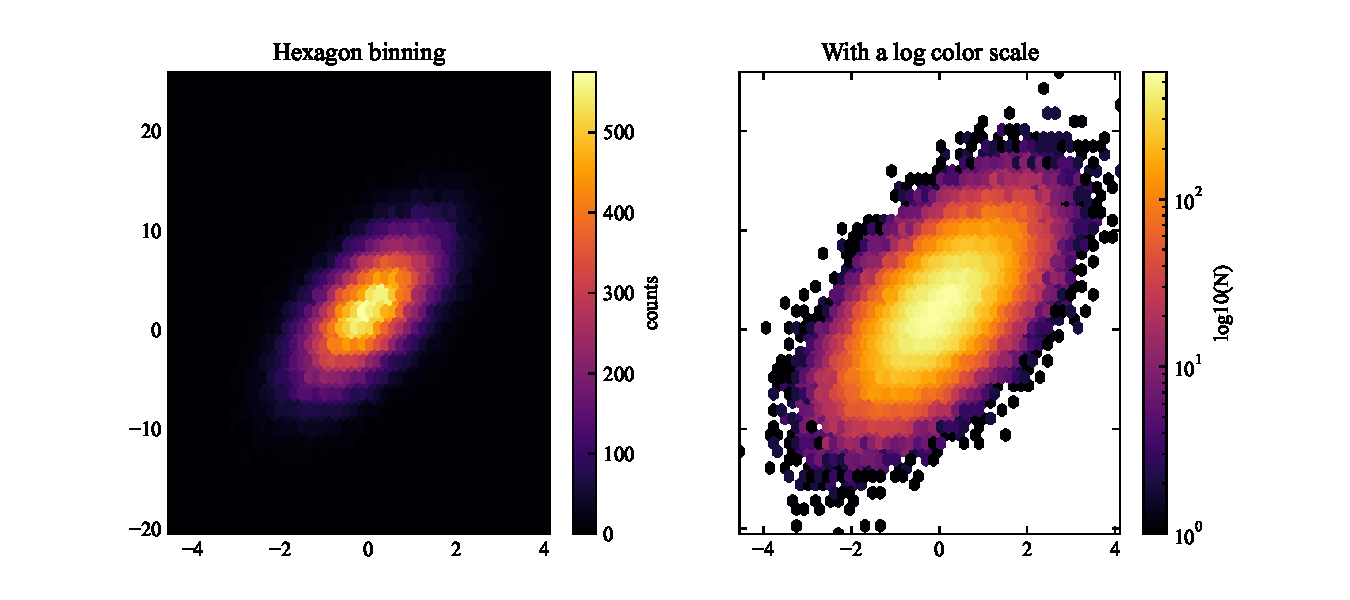
\includegraphics[width=1\textwidth]{figures/hexbin.pdf}
	\bicaption[六边形分bin图]{六边形分bin图六边形分bin图六边形分bin图六边形分bin图六边形分bin图六边形分bin图六边形分bin图六边形分bin图}[Hexagonal binned plot]
    {Hexagonal binned plot Hexagonal binned plot Hexagonal binned plot Hexagonal binned plot Hexagonal binned plot Hexagonal binned plot Hexagonal binned plot}
	\label{fig:hexbin}
\end{figure}
\begin{figure}[htbp]
	\centering
    \begin{subfigure}{0.45\textwidth}
        \centering
	    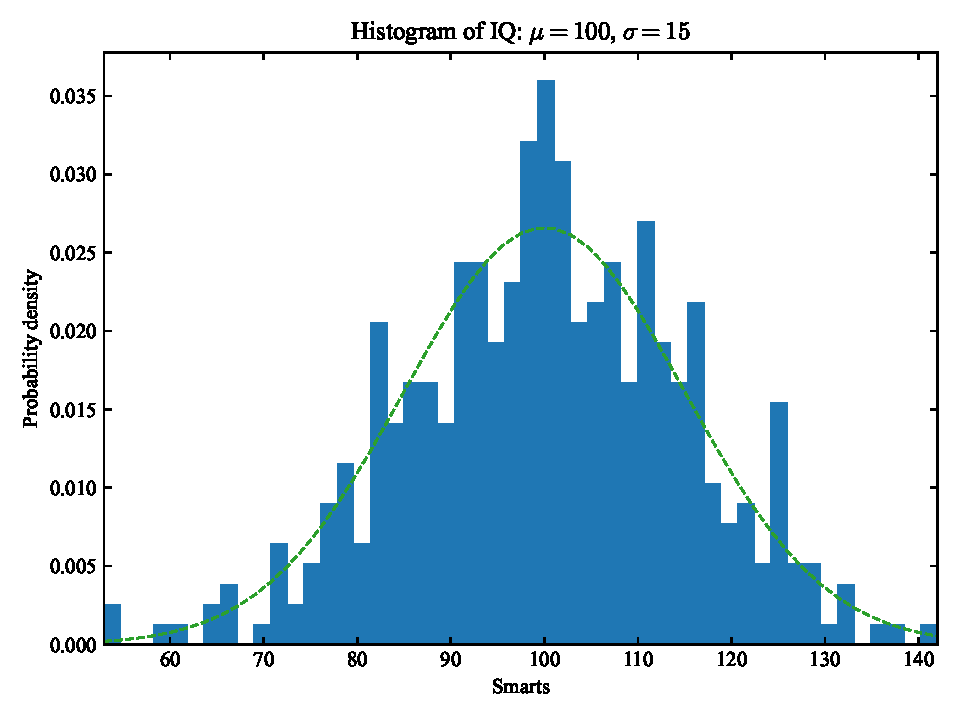
\includegraphics[width=1\textwidth]{figures/histogram.pdf}
	    \bicaption{柱状图}
        {Histogram}
    \end{subfigure}
    \begin{subfigure}{0.45\textwidth}
        \centering
	    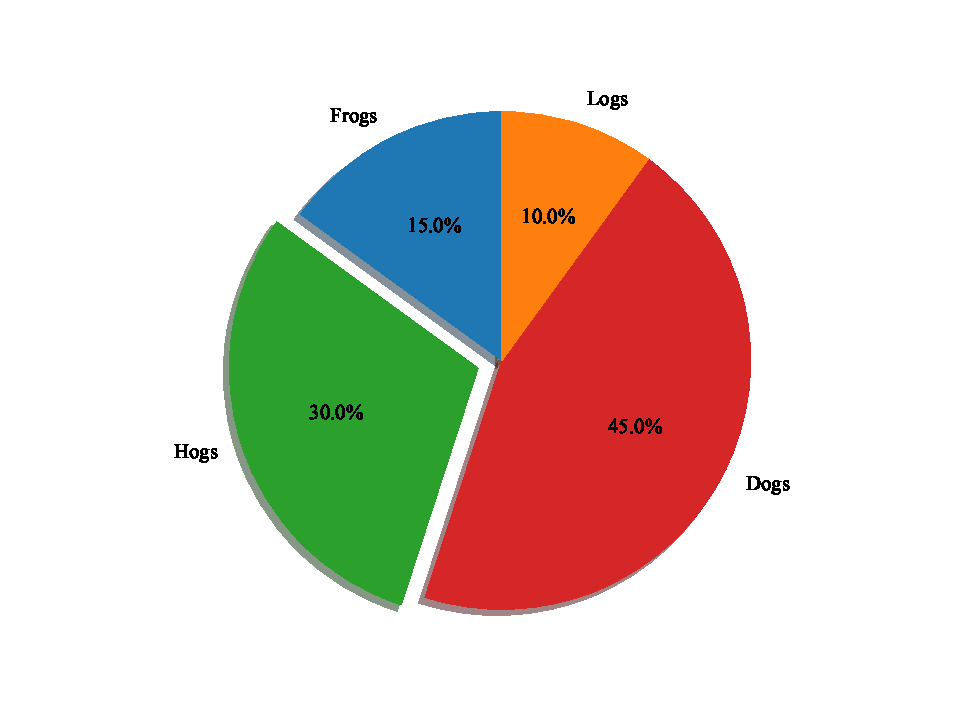
\includegraphics[width=1\textwidth]{figures/piechart.pdf}
	    \bicaption{饼状图}
        {Pie chart}
    \end{subfigure}
    \bicaption{子图示例}
    {Subfigure example}
    \label{fig:subfig}
\end{figure}

插图的引用示例:\autoref{fig:hexbin}是普通插图。

\section{表格示例}
\sectionen{Table example}

文中的表格建议使用 \texttt{table}环境里嵌套 \texttt{tabular}环境。
\begin{table}[htbp]
    \zihao{5}
    \bicaption{2022年北京冬奥会奖牌榜}
    {2022 Beijing winter Olympics medals}
    \label{tab:01}
    \centering
    \begin{tabular}{ccrrrr}
        \toprule
        总排名 & 国家/地区 & 金牌 & 银牌 & 铜牌 & 合计  \\ 
        \midrule
        1 & 挪威 & 16 & 8 & 13 & 37\\
        2 & 德国 & 12 & 10 & 5 & 27\\
        3 & 中国 & 9 & 4 & 2 & 15\\
        4 & 美国 & 8 & 10 & 7 & 25\\
        5 & 瑞典 & 8 & 5 & 5 & 18\\
        6 & 荷兰 & 8 & 5 & 4 & 17\\
        7 & 奥地利 & 7 & 7 & 4 & 18\\
        8 & 瑞士 & 7 & 2 & 5 & 14\\
        9 & 俄罗斯奥林匹克委员会\footnotemark & 6 & 12 & 14 & 32\\ 
        10 & 法国 & 5 & 7 & 2 & 14\\
        \bottomrule
    \end{tabular}
\end{table}
\footnotetext{俄罗斯由于被禁赛,不能以国家名义参加奥运会,不能使用国旗和国歌。因此俄罗斯代表团绕过禁令,以俄罗斯奥委会(Russian Olympic Committee)的名义参赛,以俄罗斯奥委会的会旗作为代表团的团旗,以柴可夫斯基的《第一钢琴协奏曲》作为团歌\cite{ROC}。}
这里需要注意,如果需要在表格内添加注释,请使用 \texttt{tablefootnote}宏包的 \texttt{\char92 tablefootnote}命令。如果要制作长表格,请使用 \texttt{longtable}宏包的 \texttt{longtable}环境,如\autoref{tab:longtable}。此外,本模版还对 \texttt{tabularray} 宏包进行了设置,可以使用 \texttt{longtblr} 环境来制作表格,如\autoref{tab:longtblr}和\autoref{tab:tblr}。\textbf{但注意:目前 \texttt{tabularray} 还未对双语标题和 List Of Tables 进行设置。}此外,在科技论文的排版中,一般使用三线表。推荐您使用 \texttt{booktabs} 宏包,该宏包支持三线表。本模版已经装载了 \texttt{booktabs} 宏包,可使用 \texttt{\char92 toprule}、 \texttt{\char92 midrule} 和 \texttt{\char92 bottomrule} 命令替换掉对应的 \texttt{\char92 hline} 即可。表格的引用示例:\autoref{tab:01}是2022年北京冬奥会奖牌榜。

{\zihao{5}%
\begin{longtable}[c]{ccc}
    \bicaption{长表格示例。\label{tab:longtable}}{Long Table Example.}\\
    
    \toprule
    Head & Head & Head \\
    \midrule
    \endfirsthead
    
    \multicolumn{3}{c}{\autoref{tab:longtable}(续)} \\
    \multicolumn{3}{c}{Table~\ref{tab:longtable}(Continued)} \\
    \toprule
    Head & Head & Head \\
    \midrule
    \endhead
    \bottomrule
    \multicolumn{3}{r}{下页续}
    
    \endfoot
    
    \bottomrule
    \endlastfoot
    
    Alpha & Beta & Gamma \\
    Epsilon & Zet & Eta \\
    Iota & Kappa & Lambda \\
    Nu & Xi & Omicron \\
    Rho & Sigma & Tau \\
    Phi & Chi & Psi \\
    Alpha & Beta & Gamma \\
    Epsilon & Zeta & Eta \\
    Iota & Kappa & Lambda \\
    Nu & Xi & Omicron \\
    Rho & Sigma & Tau \\
    Phi & Chi & Psi \\
    Alpha & Beta & Gamma \\
    Epsilon & Zeta & Eta \\
    Iota & Kappa & Lambda \\
    Nu & Xi & Omicron \\
    Rho & Sigma & Tau \\
    Phi & Chi & Psi \\
    Alpha & Beta & Gamma \\
    Epsilon & Zeta & Eta \\
    Iota & Kappa & Lambda \\
    Nu & Xi & Omicron \\
    Rho & Sigma & Tau \\
    Phi & Chi & Psi \\
    Alpha & Beta & Gamma \\
    Epsilon & Zeta & Eta \\
    Iota & Kappa & Lambda \\
    Nu & Xi & Omicron \\
    Rho & Sigma & Tau \\
    Phi & Chi & Psi \\
    Alpha & Beta & Gamma \\
    Epsilon & Zeta & Eta \\
    Iota & Kappa & Lambda \\
    Nu & Xi & Omicron \\
    Rho & Sigma & Tau \\
    Phi & Chi & Psi \\
    Foot & Foot & Foot \\
\end{longtable}
}
\begin{longtblr}[
    caption = {一个很长很长的表格示例。},
    entry = {长表格短标题},
    label = {tab:longtblr},
    note{$\dag$} = {It is a long long long long long long footnote.},
    remark{注意} = {Some general note. Some general note. Some general note.},
]{
    colspec = {XXX}, width = 0.85\linewidth,
    rowhead = 2, rowfoot = 0,
    % row{odd} = {sysugreen!50}, row{even} = {sysured!50},
    row{1-Z} = {font=\zihao{5}},
}
    \toprule
    Head & Head & Head \\
    \midrule
    Alpha & Beta & Gamma \\
    Epsilon & Zet & Eta \\
    Iota & Kappaa\TblrNote{$\dag$} & Lambda \\
    Nu & Xi & Omicron \\
    Rho & Sigma & Tau \\
    Phi & Chi & Psi \\
    Alpha & Beta & Gamma \\
    Epsilon & Zeta & Eta \\
    Iota & Kappa & Lambda \\
    Nu & Xi & Omicron \\
    Rho & Sigma & Tau \\
    Phi & Chi & Psi \\
    Alpha & Beta & Gamma \\
    Epsilon & Zeta & Eta \\
    Iota & Kappa & Lambda \\
    Nu & Xi & Omicron \\
    Rho & Sigma & Tau \\
    Phi & Chi & Psi \\
    Alpha & Beta & Gamma \\
    Epsilon & Zeta & Eta \\
    Iota & Kappa & Lambda \\
    Nu & Xi & Omicron \\
    Rho & Sigma & Tau \\
    Phi & Chi & Psi \\
    Alpha & Beta & Gamma \\
    Epsilon & Zeta & Eta \\
    Iota & Kappa & Lambda \\
    Nu & Xi & Omicron \\
    Rho & Sigma & Tau \\
    Phi & Chi & Psi \\
    Alpha & Beta & Gamma \\
    Epsilon & Zeta & Eta \\
    Iota & Kappa & Lambda \\
    Nu & Xi & Omicron \\
    Rho & Sigma & Tau \\
    Phi & Chi & Psi \\
    Foot & Foot & Foot \\
    \bottomrule
\end{longtblr}
\begin{talltblr}[
    caption = {一个正常表格示例。},
    entry = {正常表格短标题},
    label = {tab:tblr},
    note{$\dag$} = {It is a footnote.},
    remark{注意} = {Some general note. Some general note. Some general note.},
]{
    colspec = {XXX}, width = 0.85\linewidth,
    rowhead = 2, rowfoot = 0,
    row{1-Z} = {font=\zihao{5}},
}
    \toprule
    Head & Head & Head \\
    \midrule
    Alpha & Beta & Gamma \\
    Epsilon & Zet & Eta \\
    Iota & Kappa\TblrNote{$\dag$} & Lambda \\
    Nu & Xi & Omicron \\
    Rho & Sigma & Tau \\
    Phi & Chi & Psi \\
    Foot & Foot & Foot \\
    \bottomrule
\end{talltblr}

\section{其他数学环境示例}
\sectionen{Other theorem environments example}

以下是本模版预设的数学环境示例:

\begin{assumption}[连续统假设]
    不存在一个基数绝对大于可数集而绝对小于实数集的集合。
\end{assumption}
\begin{axiom}[平行公理]
    若两条直线都与第三条直线相交,并且在同一边的内角之和小于两个直角,则这两条直线在这一边必定相交。
\end{axiom}
\begin{conjecture}[黎曼猜想]
    黎曼$\zeta$函数
    \begin{align}
        \zeta(s) = \frac{1}{1^s} + \frac{1}{2^s} + \frac{1}{3^s} + \frac{1}{4^s} + \cdots
    \end{align}
    非平凡点的实数部分是$1/2$。
\end{conjecture}
\begin{definition}[定义的定义]
    对一个概念或者词或者词组的定义是描写其内涵,即描写其所有和仅有的元素的共有特征。其外延是所有这个概念、词或者词组包含的事物。
\end{definition}
\begin{example}
    举个栗子。
\end{example}
\begin{exercise}
    TiMi,发出学习的声音。
\end{exercise}
\begin{lemma}[欧几里得引理]
    如果一个正整数整除另外两个正整数的乘积,第一个整数与第二个整数互质,那么第一个整数整除第三个整数。
\end{lemma}
\begin{problem}
    花儿为什么这样红?
\end{problem}
\begin{proposition}
    通过一个不在直线上的点,有且仅有一条不与该直线相交的直线。
\end{proposition}
\begin{theorem}[诺特定理]
    对于每个局部作用下的可微对称性,存在一个对应的守恒流。另言之,每个连续对称性都有着相应的守恒定律。
\end{theorem}
\begin{corollary}
    推论往往在定理后出现。如果命题B能够被简单明了的从命题A推导出,则称B为A的推论。
\end{corollary}
\begin{solution}
    这个问题无解。
\end{solution}
\begin{proof}
    因为爱情,不会轻易悲伤,所以一切都是幸福的模样。
\end{proof}

\section{算法环境}

在论文中插入算法,我们使用的是 \texttt{algorithm2e} 宏包的 \texttt{algorithm} 环境。在 \texttt{algorithm} 环境中,你可以使用 \texttt{\char92 For}、 \texttt{\char92 While}、 \texttt{\char92 If}、 \texttt{\char92 eIF} 等命令来编写算法的结构,具体的使用方法请参考 \texttt{algorithm2e} 宏包的文档。例如\autoref{algo:algorithm} 和\autoref{algo:IR} 是算法示例。

\begin{algorithm}[htb]
    \caption{算法示例 \\ \textbf{Algorithm~\ref{algo:algorithm}:} How to write algorithms}
    \label{algo:algorithm}
    \SetAlgoLined
    \KwData{this text}
    \KwResult{how to write algorithm with \LaTeX2e }
    initialization\;
    \While{not at end of this document}{
      read current\;
      \eIf{understand}{
        go to next section\;
        current section becomes this one\;
        }{
        go back to the beginning of current section\;
        }
      }
\end{algorithm}
\begin{algorithm}[p]
    \DontPrintSemicolon
    \KwData{$G=(X,U)$ such that $G^{tc}$ is an order.}
    \KwResult{$G’=(X,V)$ with $V\subseteq U$ such that $G’^{tc}$ is an
    interval order.}
    \Begin{
    $V \longleftarrow U$\;
    $S \longleftarrow \emptyset$\;
    \For{$x\in X$}{
    $NbSuccInS(x) \longleftarrow 0$\;
    $NbPredInMin(x) \longleftarrow 0$\;
    $NbPredNotInMin(x) \longleftarrow |ImPred(x)|$\;
    }
    \For{$x \in X$}{
    \If{$NbPredInMin(x) = 0$ {\bf and} $NbPredNotInMin(x) = 0$}{
    $AppendToMin(x)$}
    }
    \nl\While{$S \neq \emptyset$}{\label{InRes1}
    \nlset{REM} remove $x$ from the list of $T$ of maximal index\;\label{InResR}
    \lnl{InRes2}\While{$|S \cap ImSucc(x)| \neq |S|$}{
    \For{$ y \in S-ImSucc(x)$}{
    \{ remove from $V$ all the arcs $zy$ : \}\;
    \For{$z \in ImPred(y) \cap Min$}{
    remove the arc $zy$ from $V$\;
    $NbSuccInS(z) \longleftarrow NbSuccInS(z) - 1$\;
    move $z$ in $T$ to the list preceding its present list\;
    \{i.e. If $z \in T[k]$, move $z$ from $T[k]$ to
    $T[k-1]$\}\;
    }
    $NbPredInMin(y) \longleftarrow 0$\;
    $NbPredNotInMin(y) \longleftarrow 0$\;
    $S \longleftarrow S - \{y\}$\;
    $AppendToMin(y)$\;
    }
    }
    $RemoveFromMin(x)$\;
    }
    }
    \caption{IntervalRestriction}
    \label{algo:IR}
\end{algorithm}

\section{代码示例}
\sectionen{Code listings example}

在论文中插入代码,我们使用的是 \texttt{listings}宏包的 \texttt{lstlisting}环境,如:
\begin{lstlisting}[language=Python,
    caption1=Python 画图代码1,
    caption2=Python ploting code 1]
import numpy as np
import matplotlib.pyplot as plt

# Fixing random state for reproducibility
np.random.seed(19680801)

dt = 0.01
t = np.arange(0, 30, dt)
nse1 = np.random.randn(len(t))                 # white noise 1
nse2 = np.random.randn(len(t))                 # white noise 2
    
# Two signals with a coherent part at 10Hz and a random part
s1 = np.sin(2 * np.pi * 10 * t) + nse1
s2 = np.sin(2 * np.pi * 10 * t) + nse2

fig, axs = plt.subplots(2, 1)
axs[0].plot(t, s1, t, s2)
axs[0].set_xlim(0, 2)
axs[0].set_xlabel('time')
axs[0].set_ylabel('s1 and s2')
axs[0].grid(True)
 
cxy, f = axs[1].cohere(s1, s2, 256, 1. / dt)
axs[1].set_ylabel('coherence')

fig.tight_layout()
plt.show()
\end{lstlisting}
或 \texttt{\char92 lstinputlisting}命令,如:
\lstinputlisting[language=Python,
    caption1=Python 画图代码2,
    caption2=Python ploting code 2,
    label=lst:cohere]
{codes/cohere.py}
代码可以使用 \texttt{caption} 选项,如果是双语标题请分别使用 \texttt{caption1} 和 \texttt{caption2}。例如\autoref{lst:cohere} 的\TeX{}源代码为:
\begin{lstlisting}[language=TeX]
\lstinputlisting[language=Python,
    caption1=Python 画图代码2,
    caption2=Python ploting code 2,
    label=lst:cohere]
{codes/cohere.py}
\end{lstlisting}

\section{参考文献}\label{sec:bibstyle}
\sectionen{References example}

\subsection{引用格式}
\subsectionen{Citation format}

\textbf{注意:本模版旧的参考文献引用格式已经弃用,转用国标,使用的是 Zeping Lee 等人开发的 \texttt{gbt7714} 宏包,具体的使用方法请参考 \url{https://github.com/zepinglee/gbt7714-bibtex-style}。}

\texttt{gbt7714} 宏包的引用标注方法与 \texttt{natbib} 宏包类似,分别有 \texttt{\char92 cite} 、\texttt{\char92 citep} 和 \texttt{\char92 citet} 三种命令,其中在顺序编码制(\texttt{numberical})中 \texttt{\char92 cite} 命令同 \texttt{\char92 citep},而在著者-出版年制(\texttt{author-year})中 \texttt{\char92 cite} 命令同 \texttt{\char92 citet}。引用有可选项,可以把引文页码放进来。此外,如果想用正文模式,还可以使用 \texttt{\char92 citestyle\{numbers\}} 命令(除非你想此后的引用标注都是正文模式,否则请用一对花括号将它的作用范围限制住,以防溢出,并且只在顺序编码制中使用)。例如:
\begin{enumerate}
    \item 这是一个期刊的引用\cite{LIGOScientific:2017zic};
    \item 这是一个加入作者的期刊引用:\citet{ZhaoWen:2017twxjz}在研究中发现……
    \item 这是一个图书的引用\cite{Rubakov:2017xzr};
    \item 这是一个加入引文页码的图书的引用\cite[92]{Zhang:2021};
    \item 这是一个研讨会论文的引用:文献{\citestyle{numbers}\cite{Tanikawa:2021+x}}中说明……
    \item 这是博士论文的引用\citep{Migenda:2019xbm,HuangGuoYuan:2020},这是硕论文的引用\citep{Shojaeifar:2015csv,SongRen:2020};
    \item 这是电子文献的引用\citep{Piro:2021oaa,bilibili:read}。
    \item 这是报纸的引用\citep{Li:2005}。
\end{enumerate}

\section{注释}
\sectionen{Remarks}

注释:可以用“脚注”或“文后注”来标注引用著作中的一些观点和案例,但全文标注方式应统一,本文统一使用“脚注”\footnote{这里是注释内容。}。注释个数不宜过多,一般不超过 10 个。
\chapter{更新描述}
\chapteren{Update Description}

\section*{\texttt{v1.1.6 2025/04/10}}
\begin{itemize}
    \item 增加摘要环境的 \texttt{noinfo} 选项,允许用户在摘要中不显示作者信息。
    \item 修复 $\hbar$ 输出错误问题,修复参考文献的引用标注排序问题。
    \item 更新查重和盲审模式下的输出,查重模式保留附录,盲审模式保留学校信息。
    \item 更新 VSCode 的 \texttt{latex-workshop} 插件的推荐配置,使用王然老师的配置\footnote{见 \url{https://github.com/OsbertWang/install-latex-guide-zh-cn}}。
\end{itemize}

\section*{\texttt{v1.1.5 2024/04/12}}
\begin{itemize}
    \item 增加了 \texttt{\char92 blindthis[<replace>]\{<content>\}} 命令,用于在盲审模式下(即 \texttt{printmode=blindmode})替换内容。在非盲审模式下,该命令不会有任何效果。在盲审模式下,该命令会将 \texttt{<content>} 替换为 \texttt{<replace>};如果直接使用 \texttt{\char92 blindthis\{<content>\}} 命令,则内容不会打印出来。
    \item 微调 \texttt{publications} 和 \texttt{achievements} 环境中标签的左边距。
\end{itemize}

\section*{\texttt{v1.1.4 2024/04/10}}
\begin{itemize}
    \item 修复了附录章在英文模式下的标签名,从 Chapter 改为 Appendix。并且新增了两个无标签章的命令 \texttt{\char92 notagchapter} 和 \texttt{\char92 notagchapteren},用于不带章节标签的章节。
    \item 对图表标题的对齐方式进行了调整,使之居中,并将之前第二标题的额外空格去除。
    \item 完善 \texttt{algorithm2e} 标题的格式,使之与图表标题一致。
\end{itemize}

\section*{\texttt{v1.1.3 2024/03/30}}
\begin{itemize}
    \item 在模板参数中对 \texttt{gbt7714} 宏包进行参数传递,可以使用著者-出版年制的参考文献格式。
    \item 使用 \texttt{algorithm2e} 宏包定制算法环境。
    \item 增加 \texttt{language} 选项,可选 \texttt{chinese} | \texttt{english} ( \texttt{<default> = chinese}),或 \texttt{zh} | \texttt{en}。如果选项为 \texttt{language=english}(或 \texttt{language=en}), 这将会将章节图表等的标题语言设置为英文。
    \item 将 \texttt{\char92 info} 命令改为 \texttt{\char92 sysuset},对模版的一些参数(如图表标签名和 \\ \texttt{acknowledgements} 环境名称等)任由用户自定义,详情见 \texttt{setup.tex} 文件。
    \item \texttt{openany}、\texttt{openright} 和 \texttt{fontset} 为 \texttt{ctexbook} 文档类的选项,不应作为模板的选项,现已移除。
    \item 撤销将 \texttt{\char92 ref} 命令的引用格式重设为 \texttt{(\char92 autoref\{key\})} 的更改。
    \item 解决了一些与 \texttt{hyperref} 宏包的冲突问题。
\end{itemize}

\section*{\texttt{v1.1.2 2024/03/14}}
\begin{itemize}
    \item 放弃自制的 \texttt{sysuthesis.bst},改用 \texttt{gbt7714} 宏包。
    \item 增加  \texttt{count\_chinese.py} Python 脚本,用于统计中文字数。
    \item 重新设置论文信息的设置方式,即键值对(key-value)的格式,更加友好。
    \item 修改了 \texttt{checkmode}的版面,去除无效的空白页。
    \item 添加了中山大学的颜色 \texttt{sysugreen}、 \texttt{sysured} 和 \texttt{spablue}。
    \item 给出了长表格的示例,并配置了 \texttt{tabularray} 的风格。
\end{itemize}

\section*{\texttt{v1.1.1 2023/03/30}}
\begin{itemize}
    \item 使用 \texttt{\char92 raggedbottom} 调整页面的垂直对齐方式, 当页面内容不足时, 这将减少页面顶部和底部之间的间距,使得页面看起来更加紧凑。
    \item 增加 \texttt{fontset} 选项 ( \texttt{<default> = fandol}),指定\CTeX{}宏集加载的字库,详情请查看\CTeX{}宏集的具体说明。例如,如果您的系统为Windows,则可以用以下选项:
\begin{lstlisting}[language=TeX]
\documentclass[doctype=thesis,printmode=final,openright,blankleft,fontset=windows]{sysuthesis}
\end{lstlisting}
    如果您在 Overleaf 上编译,则可以设置为:
\begin{lstlisting}[language=TeX]
\documentclass[doctype=thesis,printmode=final,openright,blankleft,fontset=ubuntu]{sysuthesis}
\end{lstlisting}
    目前 Mac OS 可以暂时使用 \texttt{fontset=macnew},依然解决不了找不到对应字体的警告问题,但无伤大雅。
    \item 对一些笔误进行了修改。
\end{itemize}

\section*{\texttt{v1.1.0 2023/03/03}}
\begin{itemize}
    \item 增加以下模版选项:
    \begin{itemize}
        \item \texttt{doctype},可选 \texttt{thesis}| \texttt{proposal} ( \texttt{<default> = thesis}),分别为学位论文和开题报告的格式。
        \item \texttt{printmode},可选 \texttt{final}| \texttt{checkmode}| \texttt{blindmode} ( \texttt{<default> = final}),分别为终稿、查重和盲审的打印模式。
        \item \texttt{openright}| \texttt{openany},互为 \texttt{true}| \texttt{false} ( \texttt{<default> = openright})。\\ \texttt{openright} 选项为每一章在右页(奇数页)开始, \texttt{openright} 选项为在上一章结束的下一页开始。
        \item \texttt{blankleft} ( \texttt{<default> = false}),当 \texttt{blankleft = true} 时,章节结束的偶数页如果没有内容,使之空白,但页码计数器仍然有效。
    \end{itemize}
    \item 增加了 \texttt{appendixenv}、 \texttt{publications}和 \texttt{achievements} 环境,分别为附录、学术论文发表列表和学术成果列表的环境。
    \item 对论文扉页进行了微调。
    \item 修改 \texttt{lstlisting} 双语标题格式,微调相关颜色。
    \item 增加了 NASA/ADS Export Citation 的期刊名命令,不需要再手动修改以避免 \hologo{BibTeX} 编译出错。
\end{itemize}

\section*{\texttt{v1.0.1 2022/03/06}}
\begin{itemize}
    \item 最新适配物理与天文学院的格式要求,调整了参考文献的引用格式并添加文献类型标识,将中文与西文之间的一个半角字符的自动间距关闭。 \texttt{\char92 texttt}命令只在本文档用以展示命令,不建议大家使用。
\end{itemize}

\section*{\texttt{v1.0 2022/02/23}}
\begin{itemize}
    \item 最初版本。
\end{itemize}

% 结语
% !TEX root = ../thesis.tex
\begin{conclusion}
    任何有关本模版的问题以及建议,欢迎通过以下其一方式来联系我:
    \begin{itemize}
        \item 本模版的企鹅交流群:\href{https://jq.qq.com/?_wv=1027&k=eA9mGWmS}{929324613},主要用于本模版的维护和交流,常用,能够及时回复消息;
        \item 我的个人\href{https://space.bilibili.com/326100515}{\strong{B站号}},常用,一般能很快看到消息;
        \item 我的\href{https://space.bilibili.com/326100515}{\strong{GitHub}}主页,不常用,主要用于本模版的最新版本发布。
    \end{itemize}
\end{conclusion}

% 参考文献
\makebib{refs}

% 附录
\appendix
% !TEX root = ../thesis.tex
\begin{appendixenv}
    \chapter{附录说明}
    % 使用 \chapter*{} 时,附录计数器不会增加,其中的公式图表的编号会出问题,如 (-1)。
    \chapteren{Appendix Note}
    
    附录是正文主体的补充。下列内容可以作为附录:
    \begin{enumerate}
        \item 攻读学位期间发表的(含已录用,并有录用通知书
        的)与学位论文相关的学术论文目录。
        \item 由于篇幅过大,或取材于复制件不便编入正文的材
        料、数据。
        \item 对本专业同行有参考价值,但一般读者不必阅读的
        材料。
        \item 论文中使用的符号意义、单位缩写、程序全文及有
        关说明书。
        \item 附件:计算机程序清单、软磁盘、鉴定证书、获奖
        奖状或专利证书的复印件等。
    \end{enumerate}
    
    \begin{align}
        a+b=c
    \end{align}
    
    \notagchapter{攻读学位期间发表的学术论文}
    \notagchapteren{Papers published in the period of Ph.D. education}

    \strong{根据要求,送审论文包括扉页、摘要、目录、正文和参考文献等全部内容(不包括致谢部分,论文的扉页、中英文摘要、正文以及附录部分均不得出现申请人和导师的姓名,发表论文情况仅录入期刊名称、发表年份、作者排名情况)。}

    因此,本模版提供了 \texttt{\char92 blindthis[<replace>]\{<content>\}} 命令,用于在盲审模式下(即\texttt{printmode=blindmode})替换内容。在非盲审模式下,该命令不会有任何效果。在盲审模式下,该命令会将 \texttt{<content>} 替换为 \texttt{<replace>};如果直接使用 \texttt{\char92 blindthis\{<content>\}} 命令,则内容不会打印出来。请看以下示例。
    
    \subsubsection{发表的学术论文}
    \begin{publications}
        \item \blindthis[第一作者]{XXX,XXX. Static Oxidation Model of Al-Mg/C Dissipation Thermal Protection Materials[J]}. Rare Metal Materials and Engineering, 2010\blindthis[.]{, 39(Suppl. 1): 520-524.(SCI收录,IDS号为669JS,IF=0.16)}
        \item \blindthis[第一作者]{XXX,XXX. 精密超声振动切削单晶铜的计算机仿真研究[J]}. 系统仿真学报\blindthis[.]{,2007,19(4):738-741,753.(EI收录号:20071310514841)}
        \item \blindthis[第一作者]{XXX,XXX. 局部多孔质气体静压轴向轴承静态特性的数值求解[J]}. 摩擦学学报,2007\blindthis{(1):68-72.(EI收录号:20071510544816)}
        \item \blindthis[第一作者]{XXX,XXX. 硬脆光学晶体材料超精密切削理论研究综述[J]}. 机械工程学报,2003\blindthis[.]{,39(8):15-22.(EI收录号:2004088028875)}
        \item \blindthis[第一作者]{XXX,XXX. 基于遗传算法的超精密切削加工表面粗糙度预测模型的参数辨识以及切削参数优化[J]}. 机械工程学报,2005\blindthis[.]{,41(11):158-162.(EI收录号:2006039650087)}
        \item \blindthis[第一作者]{XXX,XXX. Discrete Sliding Mode Cintrok with Fuzzy Adaptive Reaching Law on 6-PEES Parallel Robot[C]}. Intelligent System Design and Applications, Jinan, 2006\blindthis[.]{: 649-652.(EI收录号:20073210746529)}
    \end{publications}
    
    \subsubsection{申请及已获得的专利(无专利时此项不必列出)}
    \begin{achievements}
        \item \blindthis{XXX,XXX. }一种温热外敷药制备方案:中国,88105607.3[P]. 1989-07-26.
    \end{achievements}
    
    \subsubsection{参与的科研项目及获奖情况}
    
    \begin{achievements}
        \item \blindthis{XXX,XXX. }XX气体静压轴承技术研究, XX省自然科学基金项目.课题编号:XXXX.
        \item \blindthis{XXX,XXX. }XX静载下预应力混凝土房屋结构设计统一理论. 黑龙江省科学技术二等奖, 2007.
    \end{achievements}
\end{appendixenv}

% 后置部分
\backmatter

% 致谢,即后记
% !TEX root = ../thesis.tex
\begin{acknowledgements}
    后记是有关本论文情况的说明性文字,主要是交代编写过程,阐述作者的感想和体会,对有关单位或个人的致谢语等。

    本模版在编写的过程当中,遇到了不少问题,也参考了许多小组以及个人的工具和模版:
    \begin{itemize}
        \item 感谢\href{https://github.com/CTeX-org/ctex-kit}{\strong{CTeX-kit}}提供了\LaTeX{}的中文支持,其开发的\href{https://ctan.org/tex-archive/language/chinese/ctex}{\strong{CTeX}}宏集在章节格式的排版上提供了很大的方便;
        \item 感谢\href{https://www.zhihu.com/people/sgcd-33}{\strong{白鸽坐飞机}}师兄,本模版在排版上主要参考了他的中山大学研究生毕业论文模板\href{https://www.overleaf.com/latex/templates/zhong-shan-da-xue-yan-jiu-sheng-bi-ye-lun-wen-mo-ban-sysupalte/kybsnywqbcdc}{\strong{SYSUpalte}};
        \item 感谢\href{https://github.com/sjtug/SJTUThesis}{\strong{SJTUThesis}}模板的制作小组和\href{https://github.com/nanmu42}{\strong{李振楠}}(\href{https://github.com/nanmu42/CQUThesis}{\strong{CQUThesis}}),本模版在编写文档类文件的过程中主要参考了他们的成果,获益匪浅;
        \item 感谢\href{https://github.com/zepinglee}{\strong{Zeping Lee}},本模版的参考文献引用格式直接使用了他的\href{https://github.com/zepinglee/gbt7714-bibtex-style}{\texttt{gbt7714}}宏包。
    \end{itemize}
    向你们致以真诚的敬意和由衷的感谢!
\end{acknowledgements}

\end{document}